\begin{figure}[t]
\centering
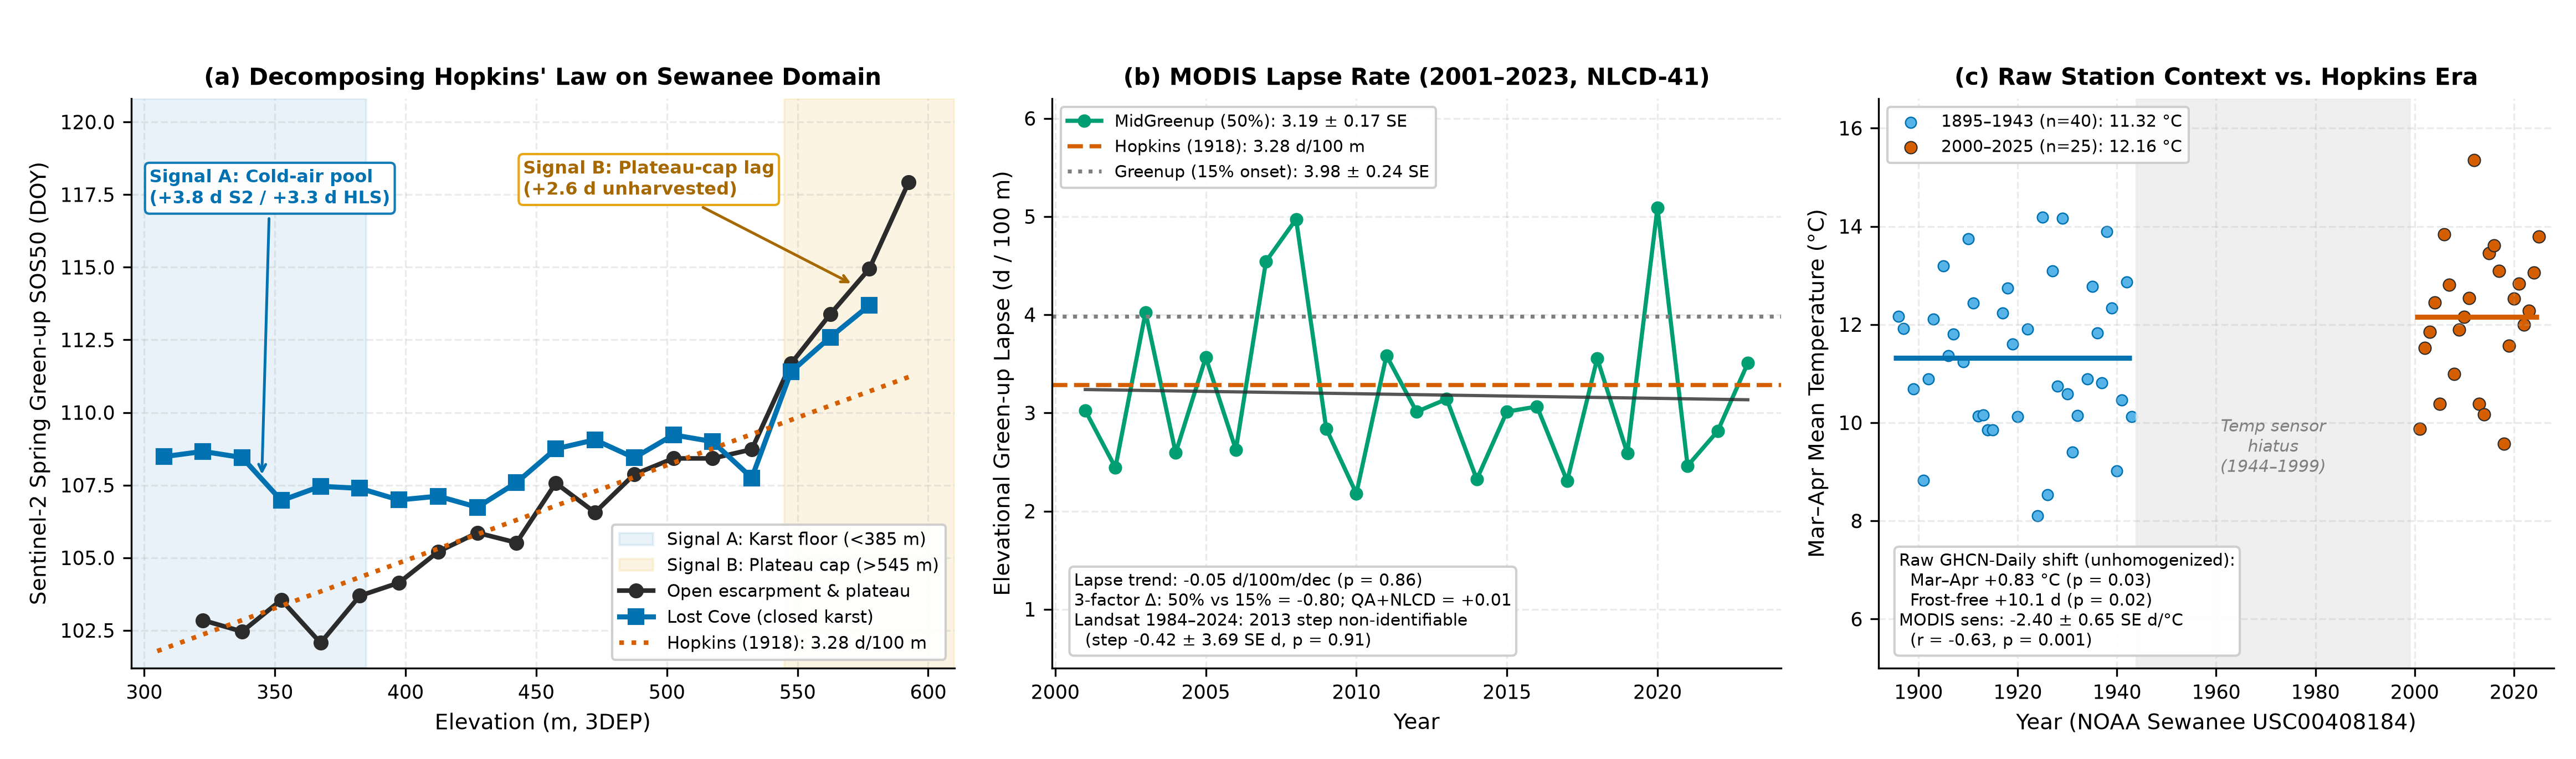
\includegraphics[width=\linewidth]{figures/fig1.png}
\caption{\textbf{Hopkins' law holds on open slopes while karst floors and flat caps bend both ends.} (a)~Sentinel-2 \texttt{SOS50} across 15~m elevation bins separates the open escarpment (black) from enclosed Lost Cove below 385~m (blue, Signal~A) and the flat plateau cap above 545~m (tan, Signal~B). (b)~Deciduous MODIS \texttt{MidGreenup\_1} (50\%, green) averages $3.19 \pm 0.17$~d/100~m (SE), matching Hopkins' 3.28 line (orange), while 15\% \texttt{Greenup\_1} (gray) averages $3.98 \pm 0.24$~d/100~m (SE). (c)~Raw, unhomogenized NOAA Sewanee records show $+0.83^\circ$C warmer March--April temperatures since 1895--1943 across the 1944--1999 sensor hiatus.}
\label{fig:hopkins_decomp}
\end{figure}
